\section{Introduction}
% make it shorter of why JavaScript is important.  
JavaScript is increasingly a popular language for software implementation: %; and the World Wide Web is increasingly an attractive platform for delivering applications.
For end users, HTML5 and its standardization enable Web apps to have an interactivity and feature-richness comparable to those implemented for traditional desktops.  
The latest round of browser wars makes executing JavaScript more efficient, robust, secure and consistent.  
For programmers, JavaScript does not have the burden of memory management and static typing; and more operating systems in both the desktop~\cite{chromeApps, windows8javascript} 
and mobile~\cite{blackberryWebWorks, firefoxOS, androidWebView, tizen} actually now support installing and running JavaScript apps on the OS similar to native apps.
The Bring Your Own Device (BYOD) movement in Enterprise IT increases hardware heterogeneity, 
which also makes JavaScript apps\footnote{JavaScript apps are preferred in Web browsers because they are lighter weight than Java applets and they don't require installation of any proprietary plugins such as Flash and Silverlight} 
a conveniently portable solution for delivering the application front end (e.g.~\cite{BNSFoffice365}).
Emergence and scalability of Node.js also make JavaScript widely adopted on the server side.  
Consequently, many institutions such as the Khan Academy~\cite{khanAcademy} use JavaScript for teaching programming; and JavaScript has consistently been a top 2 in the RedMonk~\cite{redmonk} popularity rankings.%~\footnote{results are based on projects hosted at GitHub and questions asked at StackOverflow}.

Yet, despite the language's promise and ubiquity, testing JavaScript is not easy.  
For example, because HTML describes the graphical user interface of a Web app, considerable JavaScript code is written to access and mutate HTML through the Document Object Model (DOM) API.  
When JavaScript code runs, its runtime execution would encounter DOM operations that would subtly imply the DOM tree (and thus the webpage's HTML) to have a particular structure.  
In other words, when trying to run a test case, if the DOM structure does not satisfy what the code expects it to be, execution would fail and the test case would terminate prematurely.  

\subsection{Motivating Example}
% want 1 example
% keep language consistent: DOM (not HTML). 
% give challenge numbers, approach solves challenge number say 1.  
% how to deal with incomplete traces.  concolic testing, seed.  
To further illustrate the necessity of having a satisfiable DOM structure, suppose we conduct concolic testing on the {\tt function clearBoard()} in Sample Code~\ref{dom0}.  
The function comes from a sample Web application written by Intel~\cite{mancala} for developing in the Tizen OS. 
Tizen OS

Concolic testing~\cite{cute} would execute an app in a way to maximize path coverage; to do so, we must visit both the {\tt True} and {\tt False} branches of each {\tt if} statement in Sample Code~\ref{dom0}.  
%\begin{figure}
%\begin{lstlisting}[caption=Example code whose tests and execution depend on the Document Object Model having a precise tree structure. {\tt getElementById()} is equivalent to {\tt document.getElementById()}.,label=dom0]
%function checkRows() {
%  var field = getElementById("tetris"); 
%  var i, row;
%  for (i=field.children.length; i--;) {
%    row = getElementById("row"+i);
%    if (row.children.length === 10) {
%      // ... row filled, update score
%    }
%  }
%}
%\end{lstlisting}
%\end{figure}
\begin{figure}
\begin{lstlisting}[caption=Example code whose tests and execution depend on the Document Object Model having a precise tree structure., label=dom0]
function clearBoard() {
  //clear beads
  var center = document.getElementById("center");
  var beads  = document.getElementsByClassName("beads");
  while(beads.length > 0) {
    center.removeChild(beads[0]);
    beads = document.getElementsByClassName("beads");
  }

  var beadNumber = parseInt(getBeadNumber());
  //clear text
  for(var holes=0; holes<14; holes++) {
    if (holes == 6) {
      document.getElementById("player1-score_text").innerHTML = getMessage("player_1_score")+" 0";
    }
    else if (holes == 13) {
      document.getElementById("player2-score_text").innerHTML = getMessage("player_2_score")+" 0";
    }
    else {
      document.getElementById("pit"+holes+"_count").innerText = beadNumber;
    }
  }
}
\end{lstlisting}
\end{figure}

\begin{figure*}[ht]
\centerline{\scalebox{0.25}{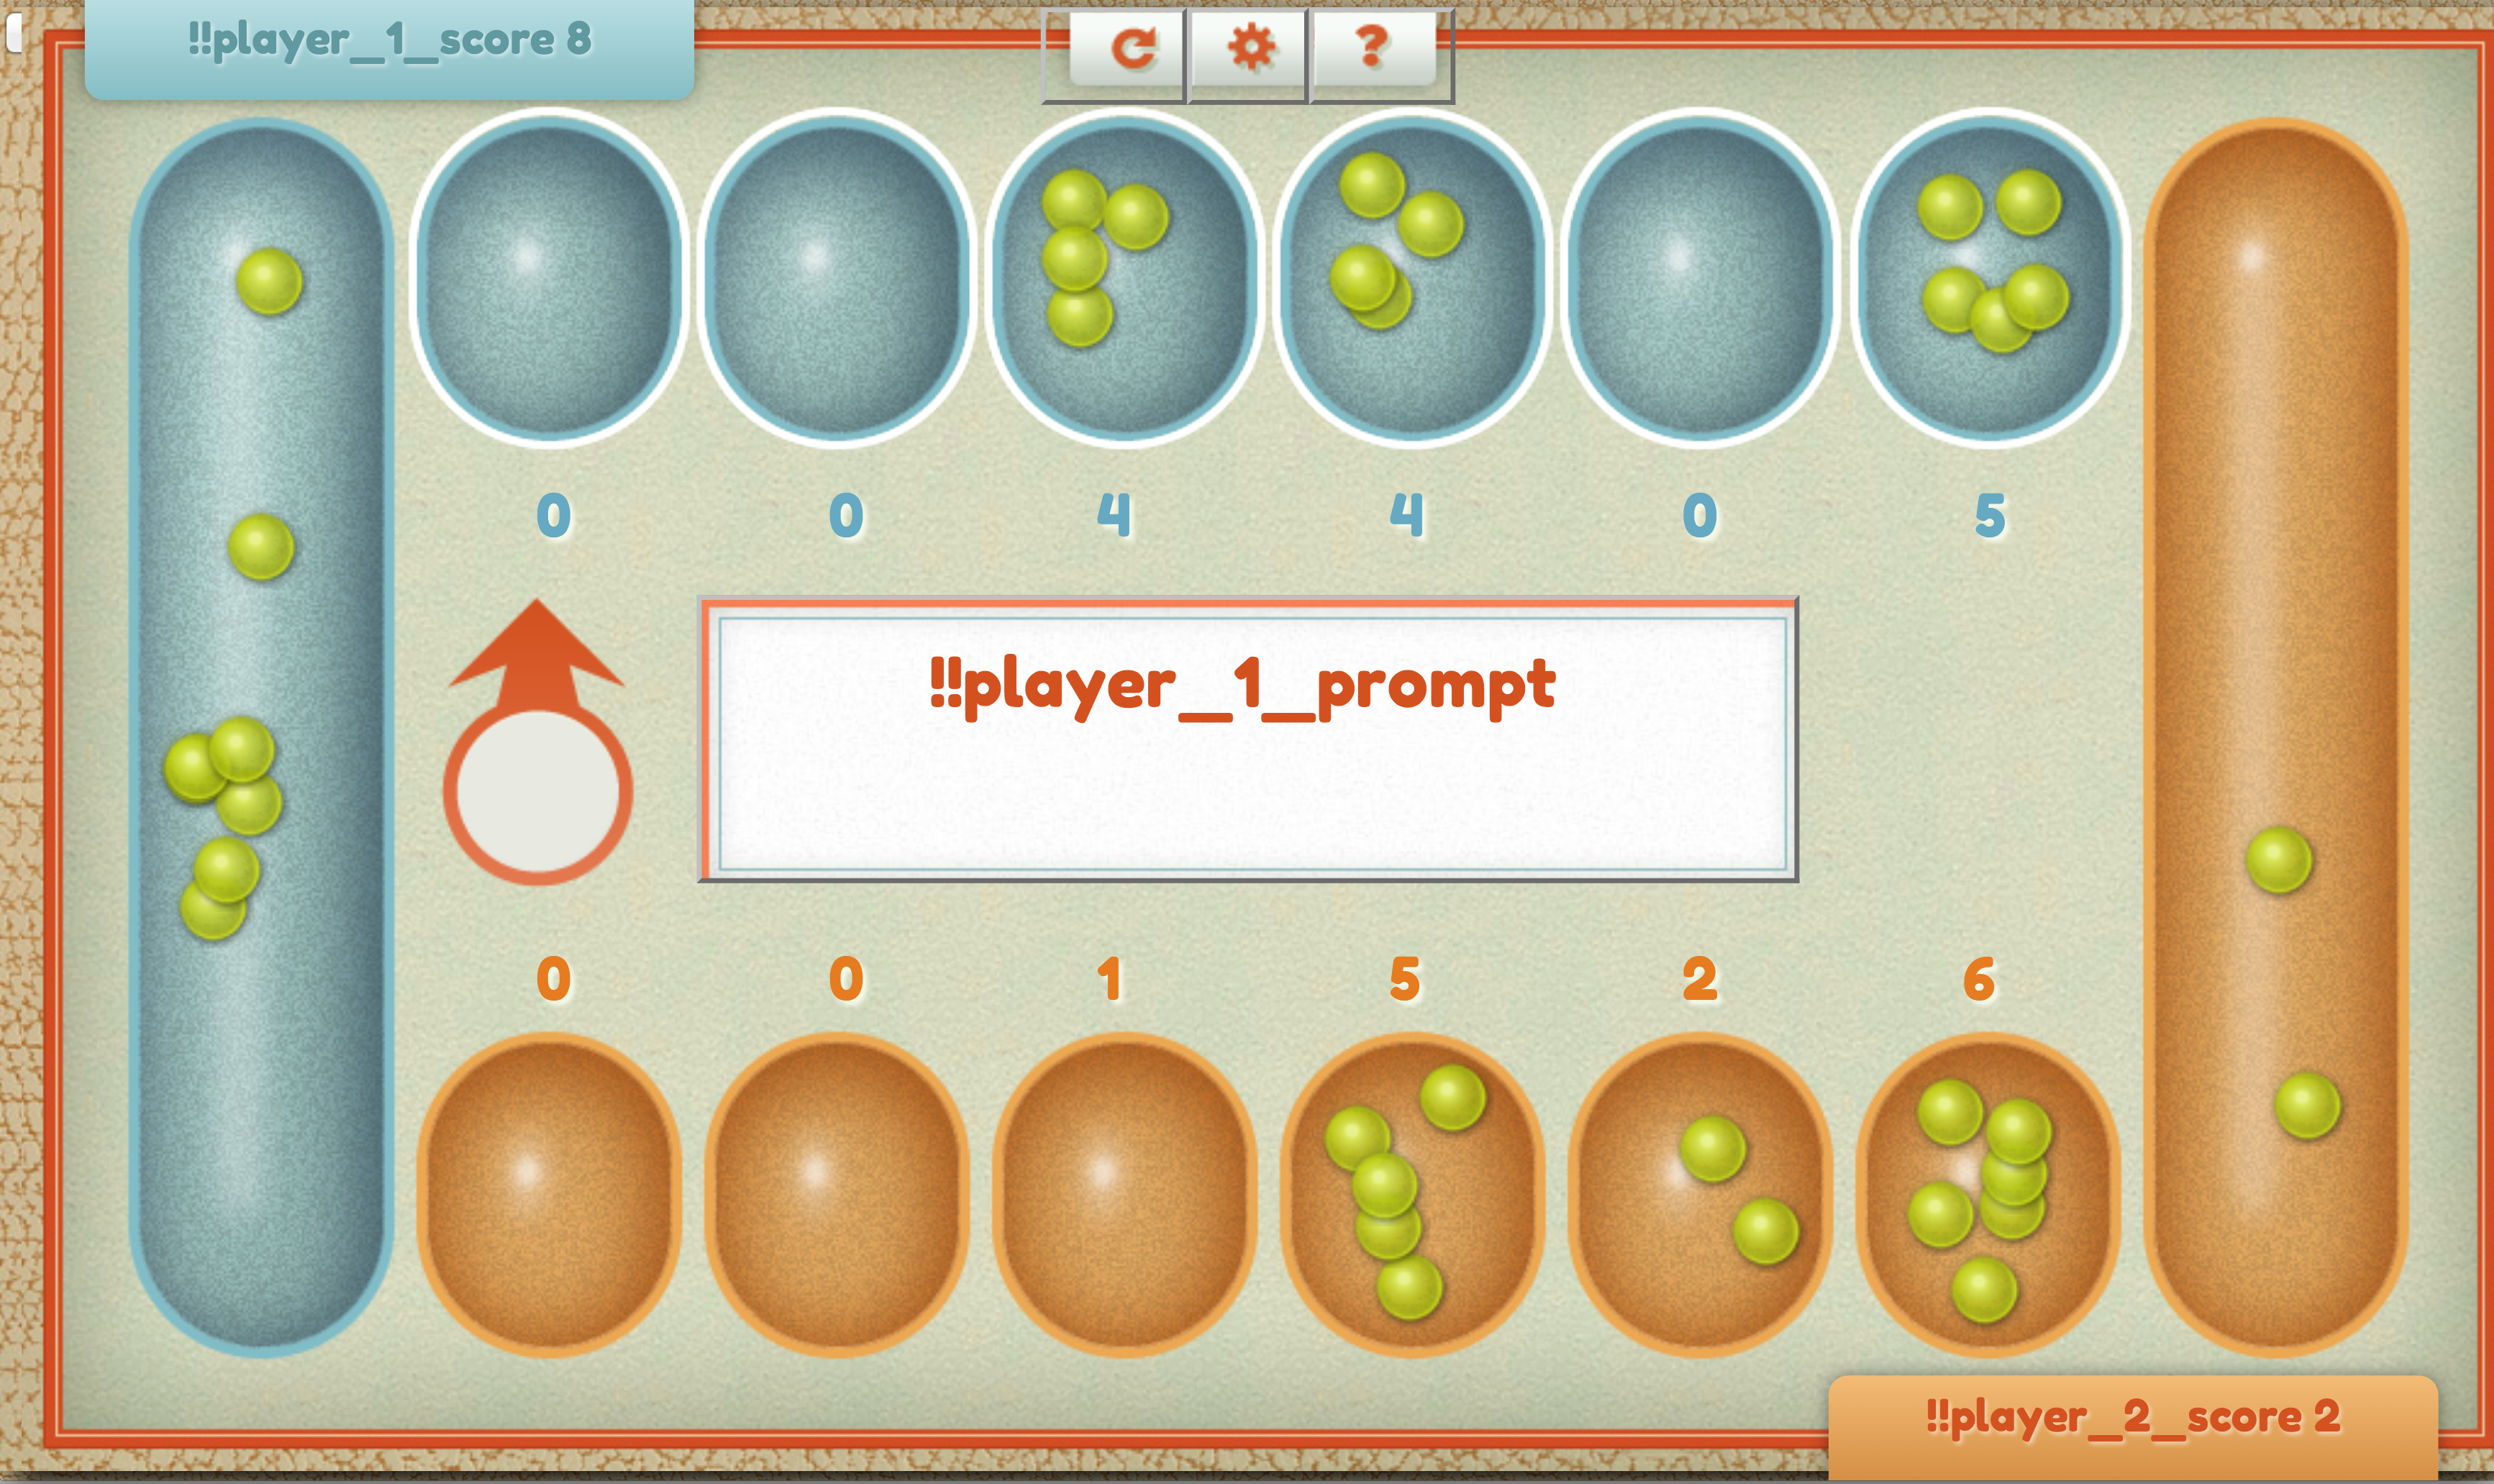
\includegraphics[natwidth=3467,natheight=2063]{mancala.png}}}
\caption[Mancala game]{}
\label{trees}
\end{figure*}

To guide the {\tt if} statement going to the {\tt True} branch, the web page's HTML must yield a DOM structure satisfying many constraints:
\begin {compactitem}
\item There is an element with id {\tt tetris}.
\item {\tt tetris} contains children elements, so that we can first enter the {\tt for} loop.
\item There are rows having id's in the nomenclature {\tt row0}, {\tt row1}, etc.
\item The number of rows must be greater than or equal to the number of children that {\tt tetris} has.  The reason is that the ID of each {\tt row} is made distinct by {\tt i}.  According to the {\tt for} loop, {\tt i---} goes from {\tt field.children.length} to 1.
\item At least one of the rows must have exactly 10 children.
\end {compactitem}

Until all of the above constraints are satisfied, the function's execution would likely lean towards an unintended path or would even halt.   
For example, when {\tt field} is {\tt null}, the property access {\tt field.children} would result in a {\tt Type Error} and consequently the rest of the function cannot be run or tested.  
Therefore, a satisfying HTML must be generated to yield a proper DOM structure so that execution of the function and of the test case would not crash and can be guided towards the intended path.  

While manual generation of HTML is possible, the manual approach would quickly become tedious and not scalable.  
The reason is that a unique DOM structure is required for going through a different execution path.
For example, to go to the {\tt False} branch of the above {\tt if}, rows cannot have 10 children.
Therefore, to cover both the {\tt True} and {\tt False} branches of an {\tt if}, we must generate 2 unique DOM structures.  
Generally in an {\tt if } block, the exact number of unique DOM structures per condition is 2 plus the number of {\tt else if}'s in the {\tt if} block.  
Loops are more difficult for achieving path coverage, because it's not easy to determine the max upper limit of loop iterations.  For example, in Sample Code ~\ref{dom0}, {\tt field} can have any number of children.

Nevertheless, the number of unique DOM structures would at least double whenever we try to cover an additional DOM-dependent condition, be it an {\tt if} or a {\tt loop}.  
Moreover, manual generation can become complex as DOM-dependent conditions can get scattered across multiple files in the code, making it labor intensive to accurately trace all of the DOM elements and relevant constraints.  
Random generation is simply not desirable because the required DOM tree may have a structure too precise for a random tree to match by chance.  
Thus the desired approach has to be automated, systematic and precise.


\subsection{Contributions}
The following are the main contributions of our paper:
\begin {compactitem}
\item We propose an automated, generic, transparent and browser-independent approach for systematically generating HTML to test JavaScript code that contains DOM operations.
\item We describe how JavaScript code and its execution can dynamically be analyzed for deducing constraints relevant for generating HTML.
\item We design a novel DOM solver for generating satisfiable a DOM tree that would yield an HTML for going into a specific execution path. 
\item We present the implementation of our approach in a tool called \tool; an online video provides a demonstration.
\item We report how \tool and its generated DOM trees can help test suites improve coverage and reach complete execution.  If a function cannot be fully executed, the test case's assertions cannot be fully run.  
\end {compactitem}

\tool augments approaches that aim to generate tests automatically.  
Random testing(e.g.~\cite{artemis}), feedback directed testing (e.g.~\cite{feedbackConcolic}), mutation testing (e.g.~\cite{pythia}), concolic testing (e.g.~\cite{cute, jalangi, kudzu, eventConcolic})... 
to our best knowledge, almost all of existing research on test generation focused on generating 1) function arguments for unit testing, or 2) events and UI inputs (e.g strings for text fields and forms; mouse clicks for buttons and selection boxes; and key presses) for application-level testing.
However, having just the function arguments, events and UI inputs is often insufficient.  For example, in a Web app, a properly satisfied dependency such as the DOM is often necessary for test cases and assertions to reach complete execution.  

Moreover, it should be noted that the {\tt function checkRows()} does not take any function arguments; and functions without input arguments are common in JavaScript.
Yet, these functions depend on major dependencies such as the DOM.
Thus even when we have a very well defined test suite, either through manual or automatic generation, considerable JavaScript code may not get properly tested and covered unless the corresponding DOM structure is available.  
\tool provides an automated and systematic solution for generating satisfiable DOM trees.  

% present emprical results

% cannot generate HTML for game, 
%Note that the code does not imply the following, which we take for granted in a Tetris game.
%\begin {compactitem}
%\item Each {\tt row} is a child element of {\tt tetris}.
%\item Each {\tt row} is vertically stacked: {\tt row10} is right above {\tt row9}, which is also right on top of {\tt row8}, and so on.
%\item Children of a {\tt row} are blocks that make up a piece.  
%\item etc.
%\end {compactitem}

